%%%%
%% TEMPLATE HW3 2017-2018
%%%%

\documentclass[addpoints,10pt,answers]{exam}
\usepackage{enumerate}
\usepackage{mathtools}
\usepackage{blkarray}
\usepackage{tikz}
   
%%%%
% IMPORTANT: YOU SHOULD INSTANTIATE THE FOLLOWING THREE COMMANDS WITH YOUR OWN INFORMATION
\newcommand{\studentonename}{Naldi Gega}     %%% Student one: first and last name
\newcommand{\studentonenumber}{S3154416}  %%% Student one: student number
\newcommand{\studenttwoname}{Gionanidis Emmanouil}     %%% Student two: first and last name
\newcommand{\studenttwonumber}{S3542068}  %%% Student two: student number
\newcommand{\ourdsgroup}{29}         %%% The number of your DS group in Nestor
%%%%


%%%% DO NOT MODIFY 
\newcommand{\hwn}{3}
\pagestyle{headandfoot}
\runningheadrule
\firstpageheader{Discrete Structures (2017-18)}{{\textbf{Answers to Homework No. \hwn}}}{\today}
\runningheader{Discrete Structures (2017-18)}
              {DS Group No.~\ourdsgroup~---~HW\hwn}
              {Page \thepage\ of \numpages}
\firstpagefooter{}{}{}
\runningfooter{}{}{}
 
  \begin{document}
 \boxedpoints
\begin{center}
  \fbox{\fbox{\parbox{5.9in}{\centering
  {\large
  \studentonename~(\studentonenumber) \& \studenttwoname~(\studenttwonumber)  \\
  DS Group No.~\ourdsgroup  }}}
 }
\end{center}
%%%% DO NOT MODIFY  


\begin{questions}

%%%%%%%%%%%%%%%%%%%%%%%%%%%%%%%%%%%%%%%%%%%%%%%%%%%%%%%
\question Question 1:
%%% INSERT YOUR SOLUTIONS HERE
%%%%>>>>>>>>>>>>>>>>>>>>>>>>>>>>>>>>>>
\begin{solution}
\\a) 3\\
b) 1\\
c) 3\\
d) 1
\end{solution}
%%%%<<<<<<<<<<<<<<<<<<<<<<<<<<<<<<<<<<
%%%%%%%%%%%%%%%%%%%%%%%%%%%%%%%%%%%%%%%%%%%%%%%%%%%%%%%


%%%%%%%%%%%%%%%%%%%%%%%%%%%%%%%%%%%%%%%%%%%%%%%%%%%%%%%
\question Question 2:
%%% INSERT YOUR SOLUTIONS HERE
%%%%>>>>>>>>>>>>>>>>>>>>>>>>>>>>>>>>>>
\begin{solution}
\\a) $A_1 \rightarrow$ 5,8 $A_2 \rightarrow$ 4,5,6,8,9\\
b) $A_1 \rightarrow$ 1,2,3 $A_2 \rightarrow$ 2\\
c) $A_1 \rightarrow$ none $A_2 \rightarrow$ none\\
d) $A_1 \rightarrow$ 3 $A_1 \rightarrow$ 2
\end{solution}
%%%%<<<<<<<<<<<<<<<<<<<<<<<<<<<<<<<<<<
%%%%%%%%%%%%%%%%%%%%%%%%%%%%%%%%%%%%%%%%%%%%%%%%%%%%%%%


%%%%%%%%%%%%%%%%%%%%%%%%%%%%%%%%%%%%%%%%%%%%%%%%%%%%%%%
\question Question 3:
%%% INSERT YOUR SOLUTIONS HERE
%%%%>>>>>>>>>>>>>>>>>>>>>>>>>>>>>>>>>>
\begin{solution}
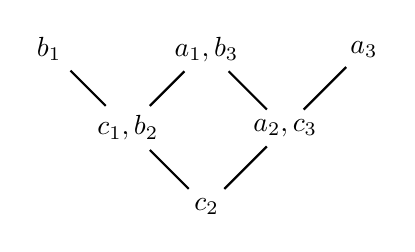
\begin{tikzpicture} 
\node (mid) at (0,0) {$a_1,b_3$};
\node [left  of=mid] (left)  {};
\node [left  of=left] (Fleft)  {$b_1$};
\node [right of=mid] (right) {};
\node [right of=right] (Fright) {$a_3$};
\node [below of=left] (Bleft)  {$c_1,b_2$};
\node [below of=right] (Bright) {$a_2,c_3$};
\node [left of=Bright] (lol) {};
\node [below of=lol] (bot) {$c_2$};
\draw [black,  thick] (Fright) -- (Bright);
\draw [black,  thick] (Bright) -- (bot);
\draw [black,  thick] (Bright) -- (mid);
\draw [black,  thick] (mid) -- (Bleft);
\draw [black,  thick] (Fleft) -- (Bleft);
\draw [black,  thick] (Bleft) -- (bot);
\end{tikzpicture}\\
\end{solution}
%%%%<<<<<<<<<<<<<<<<<<<<<<<<<<<<<<<<<<
%%%%%%%%%%%%%%%%%%%%%%%%%%%%%%%%%%%%%%%%%%%%%%%%%%%%%%%


%%%%%%%%%%%%%%%%%%%%%%%%%%%%%%%%%%%%%%%%%%%%%%%%%%%%%%%
\question Question 4:
%%% INSERT YOUR SOLUTIONS HERE
%%%%>>>>>>>>>>>>>>>>>>>>>>>>>>>>>>>>>>
\begin{solution}
\\\\ a)Lattice of $ N^+ $ with usual order $ \leq $ \\
Since $ N^+ $ contains only positive natural numbers, the least element is 1 and then it goes to infinity so there is no greatest element.\\
\\b)Lattice of $ N^- $ with usual order $ \geq $\\
This is the opposite of case a) where -1 is the greatest element but there is no least element since it decreases to infinity.\\
\\c)A poset $ A=\{ x|x\in R $ (real numbers) and $ -1\leq x\leq 1\} $ with usual order $ \leq $\\
The least element is -1 and the greatest is 1 but since $ x\in R $ there are infinite numbers between -1 and 1.
\end{solution}
%%%%<<<<<<<<<<<<<<<<<<<<<<<<<<<<<<<<<<
%%%%%%%%%%%%%%%%%%%%%%%%%%%%%%%%%%%%%%%%%%%%%%%%%%%%%%%


%%%%%%%%%%%%%%%%%%%%%%%%%%%%%%%%%%%%%%%%%%%%%%%%%%%%%%%
\question Question 5:
%%% INSERT YOUR SOLUTIONS HERE
%%%%>>>>>>>>>>>>>>>>>>>>>>>>>>>>>>>>>>
\begin{solution}
We will follow the OP's strategy and prove the following contrapositive form of the statement:

If a lattice is complemented and distributive, then every element of the lattice has a unique complement.

Convince yourself that this is equivalent to the claim in the question.

A complemented and distributive lattice is a boolean algebra, so we will use +
and ⋅ in place of ∨ and ∧

respectively. Now, of course, every element does have a complement (by definition); the real task is to show uniqueness.

Let x
be an arbitrary element, and let y and z be its complements. We want to show that $y=z$. We start from
$y=y⋅1$,
and replace 1 by $x+z$. Then applying distributivity and the fact that $yx=0$, we get
$y=y(x+z)=yx+yz=0+yz=yz$.(1)
Repeating this argument after switching y and z, we get
$z=zy$.(2)
Comparing (1) and (2), we are done. 
\\The conclusion is that  that any x in a complemented distributive lattice cannot have two complements . Also because the lattice is complemented that means that every element in the set has precisely one complement.
\end{solution}
%%%%<<<<<<<<<<<<<<<<<<<<<<<<<<<<<<<<<<
%%%%%%%%%%%%%%%%%%%%%%%%%%%%%%%%%%%%%%%%%%%%%%%%%%%%%%%


%%%%%%%%%%%%%%%%%%%%%%%%%%%%%%%%%%%%%%%%%%%%%%%%%%%%%%%
\question Question 6:
%%% INSERT YOUR SOLUTIONS HERE
%%%%>>>>>>>>>>>>>>>>>>>>>>>>>>>>>>>>>>
\begin{solution}
We will construct a function from the natural numbers onto a distributive lattice, namely the lattice of all infinite sequences of natural numbers, all but finitely many of which are 0, with coordinatewise maximum as the join and coordinatewise minimum as the meet. The function is a lattice isomorphism. Let p1,p2,… be all prime numbers indexed in order. If

$n=pi_[11]pi_[22]⋯
map n↦(i1,i2,i3,…)$

. Then this is a lattice homomorphism, join corresponds to LCM and meet corresponds to GCD.

If you can't use this answer directly, consider this as a hint that LCM means you are taking the maximum of all powers of particular primes among the two numbers and GCD means you're taking the minimum.
\end{solution}
%%%%<<<<<<<<<<<<<<<<<<<<<<<<<<<<<<<<<<
%%%%%%%%%%%%%%%%%%%%%%%%%%%%%%%%%%%%%%%%%%%%%%%%%%%%%%%



%%%%%%%%%%%%%%%%%%%%%%%%%%%%%%%%%%%%%%%%%%%%%%%%%%%%%%%
\question Question 7:
%%% INSERT YOUR SOLUTIONS HERE
%%%%>>>>>>>>>>>>>>>>>>>>>>>>>>>>>>>>>>
\begin{solution}
Assuming we have to matrices 
$$
M=
\begin{bmatrix}
	m_{11}       & m_{12}  \\
	m_{21}       & m_{22} \\
\end{bmatrix}
$$
and another one:
$$
N=
\begin{bmatrix}
	n_{11}       & n_{12} \\
	n_{21}       & n_{22} \\
\end{bmatrix}
$$

Matrices M,N are isomorphic to the same boolean algebra , so they are isomorphic to each other. We have to map the elements of the two matrices into another matrix using bijection F.Let's assume that $F(i,j) = m_[ij] - n_[ij]$ because we want $m_[ij] \leq n_[ij] => m_[ij] - n_[ij] \leq 0 $. As concern the function we $F(i,j) \leq 0 $ the assumption is True and if $0\leq F(i,j)$ the assumption is False.\\
With this way we build the matrix . So 1 implies $m_[ij]\leq n_[ij]$ and 0 the reverse . With this we express the A matrix as a boolean algebra matrix.
\end{solution}
%%%%<<<<<<<<<<<<<<<<<<<<<<<<<<<<<<<<<<
%%%%%%%%%%%%%%%%%%%%%%%%%%%%%%%%%%%%%%%%%%%%%%%%%%%%%%%


%%%%%%%%%%%%%%%%%%%%%%%%%%%%%%%%%%%%%%%%%%%%%%%%%%%%%%%
\question Question 8:
%%% INSERT YOUR SOLUTIONS HERE
%%%%>>>>>>>>>>>>>>>>>>>>>>>>>>>>>>>>>>
\begin{solution}
(a)\\$x \lor y \lor z = (x' \land y' \land z' )'$ De Morgan's Law\\\\

(b)\\$ x \lor ( y' \land ( x' \lor z )) = \\
(x \lor y)\land(x \lor x') \lor (x \lor y')\land(x \lor z) = $
(as we know from the theory $(x \lor x') = 1$)\\
$(x \lor y') \land 1 \lor (x \lor y')\land(x \lor z)$(1)
here we have to consider the procedure of absorption . An example given , assuming $x \lor y' = m$ and $x \lor z = n$ , we have $m \lor m \land n = $\\
$m \land 1 \lor m \land n=$\\
$m \land (1 \lor n)=$\\
$m$. We are going to use the same procedure with our example.\\

Continuing the procedure (1)
$(x \lor y')\land(1 \lor (x \lor z))=$\\
$(x \lor y')=$            (using De Morgan's Law)\\
$(x' \land y)'$\\\\

(c)\\
$x'\land(x \lor y \lor z)=$\\
$x'\land x \lor x' \land y \lor x' \land z=(x \land x' =0$              this is know from the axioms )\\
$x' \land (y \lor z)= $         (De Morgan's Law)\\
$x'\land(y'\land z')'$

\end{solution}
%%%%<<<<<<<<<<<<<<<<<<<<<<<<<<<<<<<<<<
%%%%%%%%%%%%%%%%%%%%%%%%%%%%%%%%%%%%%%%%%%%%%%%%%%%%%%%


 


\end{questions}
\end{document}